\chapter{PROSEDUR OPERASI}

Untuk menggunakan aplikasi ini, caranya cukup mudah, hanya dengan melakukan akses ke alamat http://bppkad.brebeskab.go.id menggunakan \textit{browser} apapun, kemudian akan muncul tampilan seperti gambar \ref{fig:main-fe} berikut ini :

\begin{figure}[H]
	\centering
	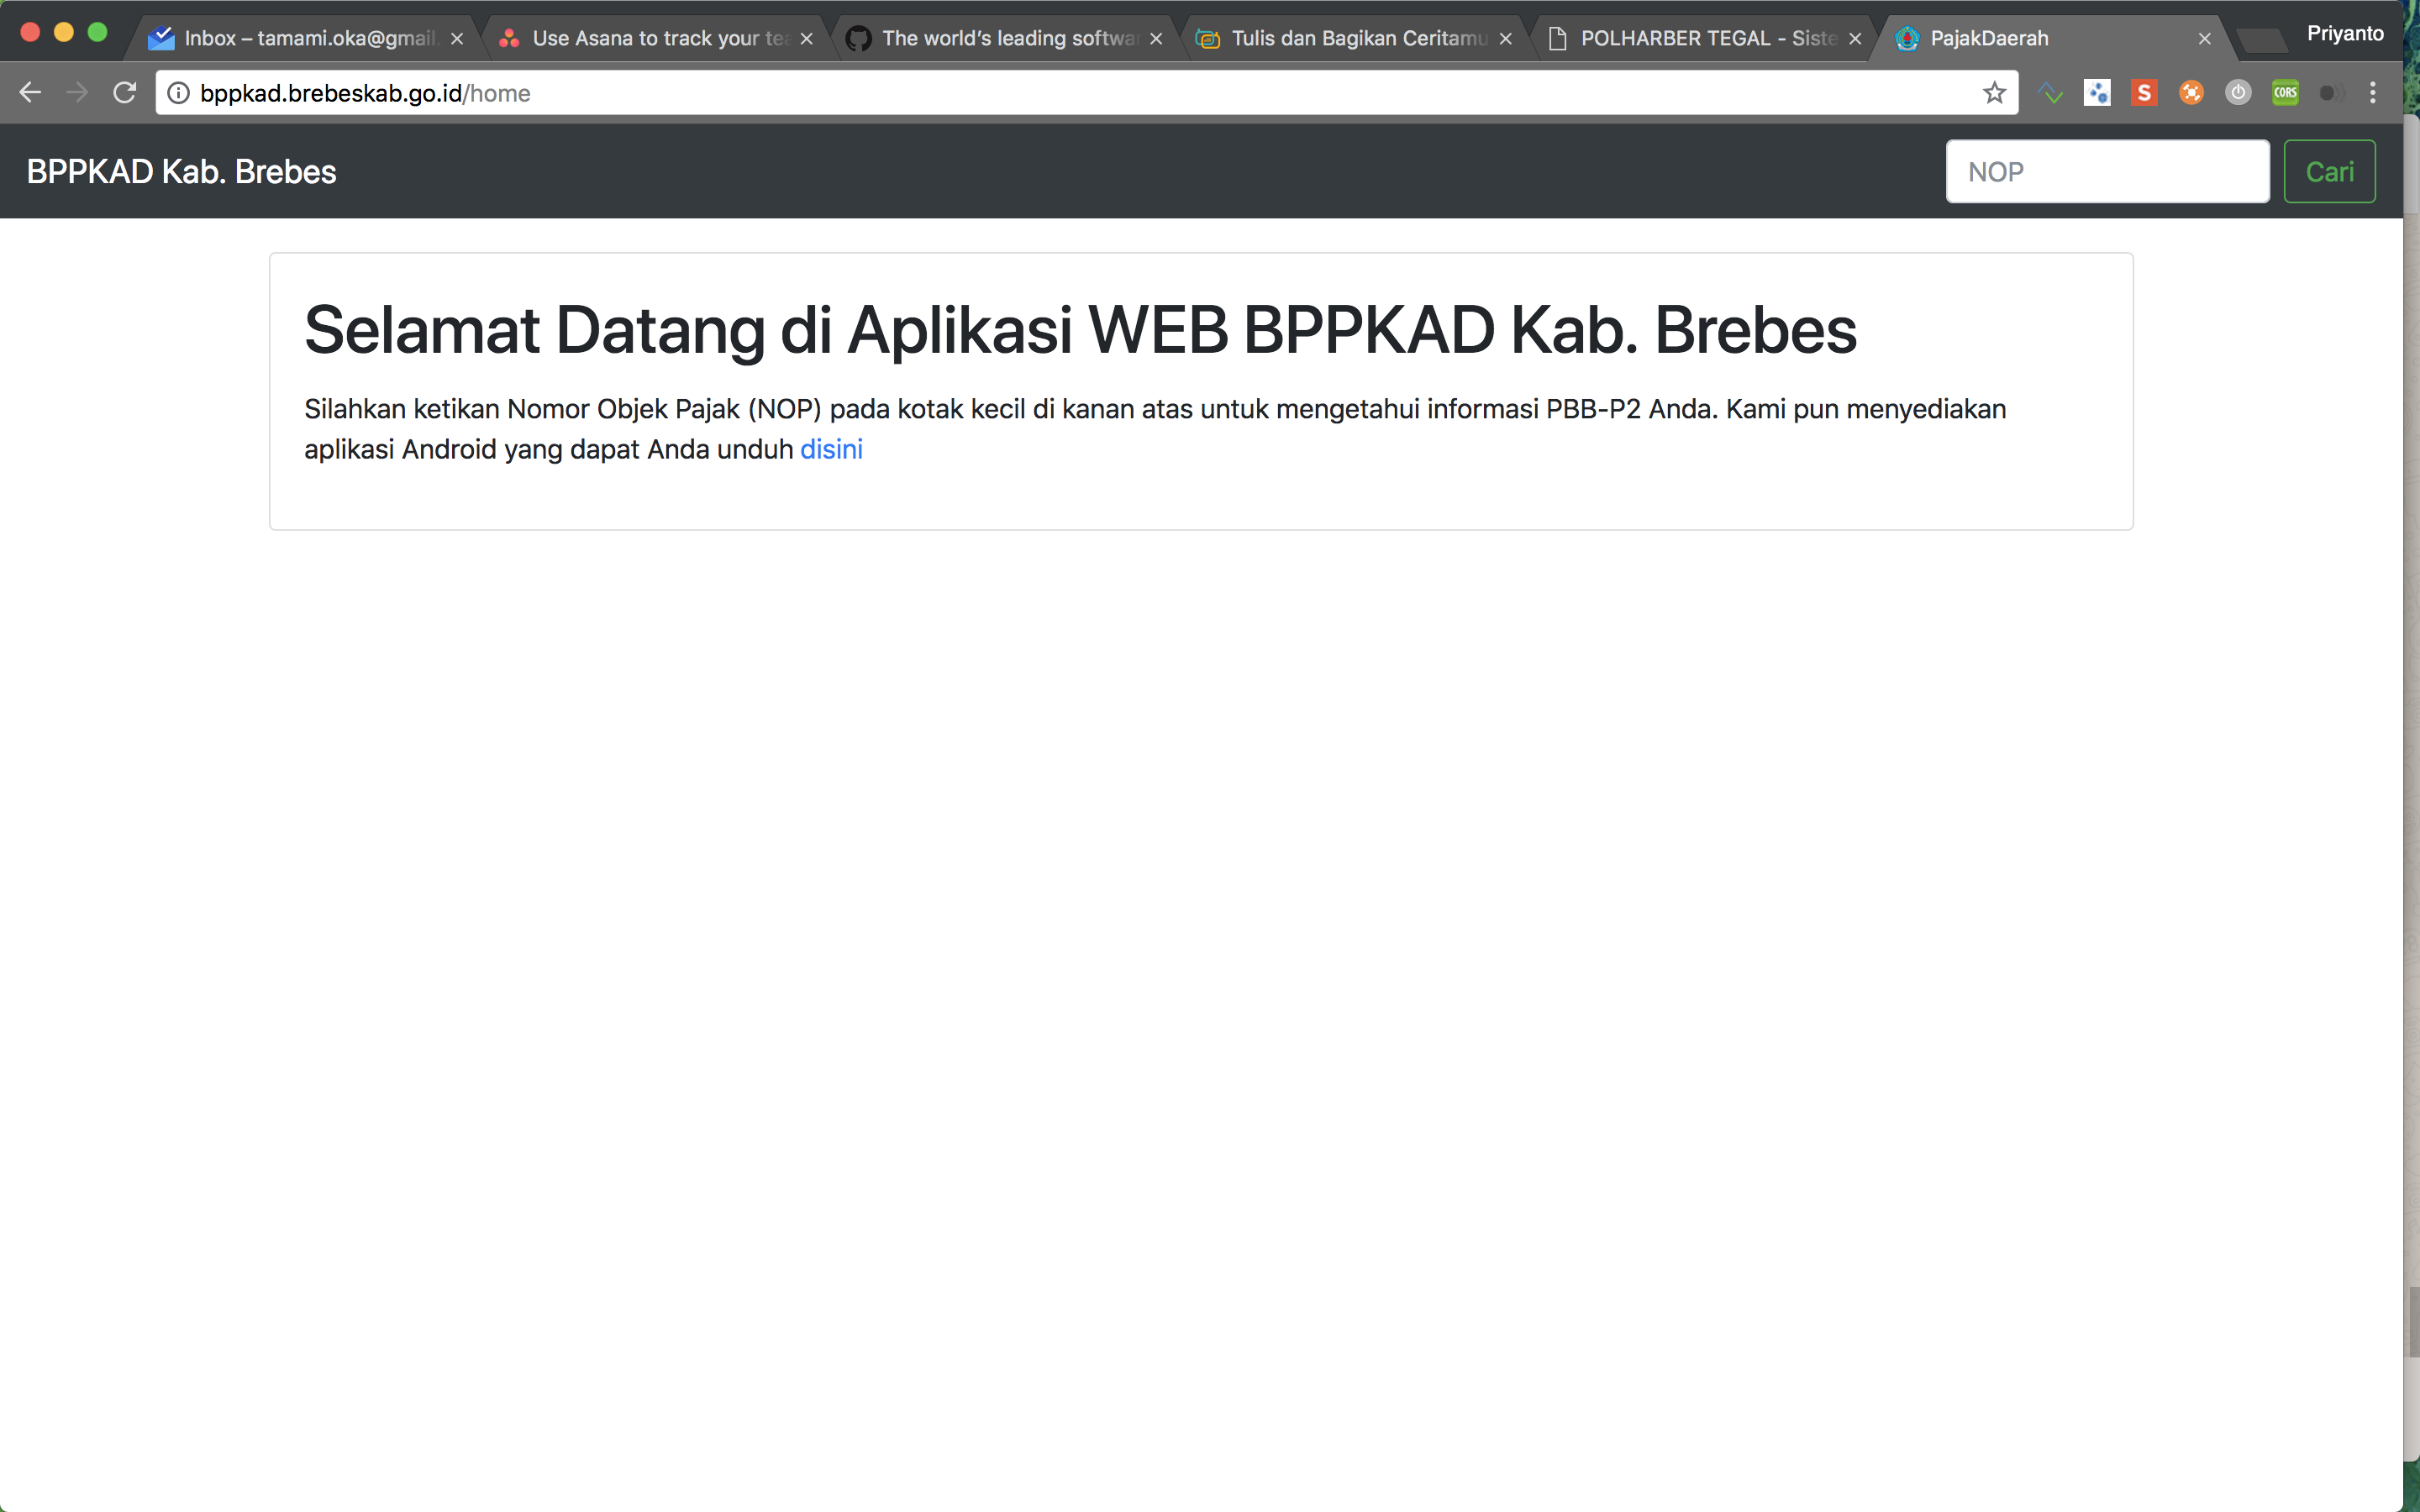
\includegraphics[width=1\textwidth]{./resources/main-fe}
	\caption{Tampilan Utama Aplikasi}
	\label{fig:main-fe}
\end{figure}

Pengguna tinggal memberikan Nomor objek Pajak (NOP) pada tempat yang telah disediakan di sebelah kanan atas halaman ini, Nomor Objek Pajak (NOP) adalah nomor yang tertera di sebelah kiri atas lembar Surat Pemberitahuan Pajak Terhutang (SPPT).

Aturan penulisan Nomor Objek Pajak (NOP) pada aplikasi ini tidak perlu menggunakan tanda baca seperti yang tertera pada lembar Surat Pemberitahuan Pajak Terhutang (SPPT), namun cukup untuk memasukkan atau mengetikkan angkanya saja, seperti contoh pada gambar \ref{fig:contoh-nop} berikut ini :

\begin{figure}[H]
	\centering
	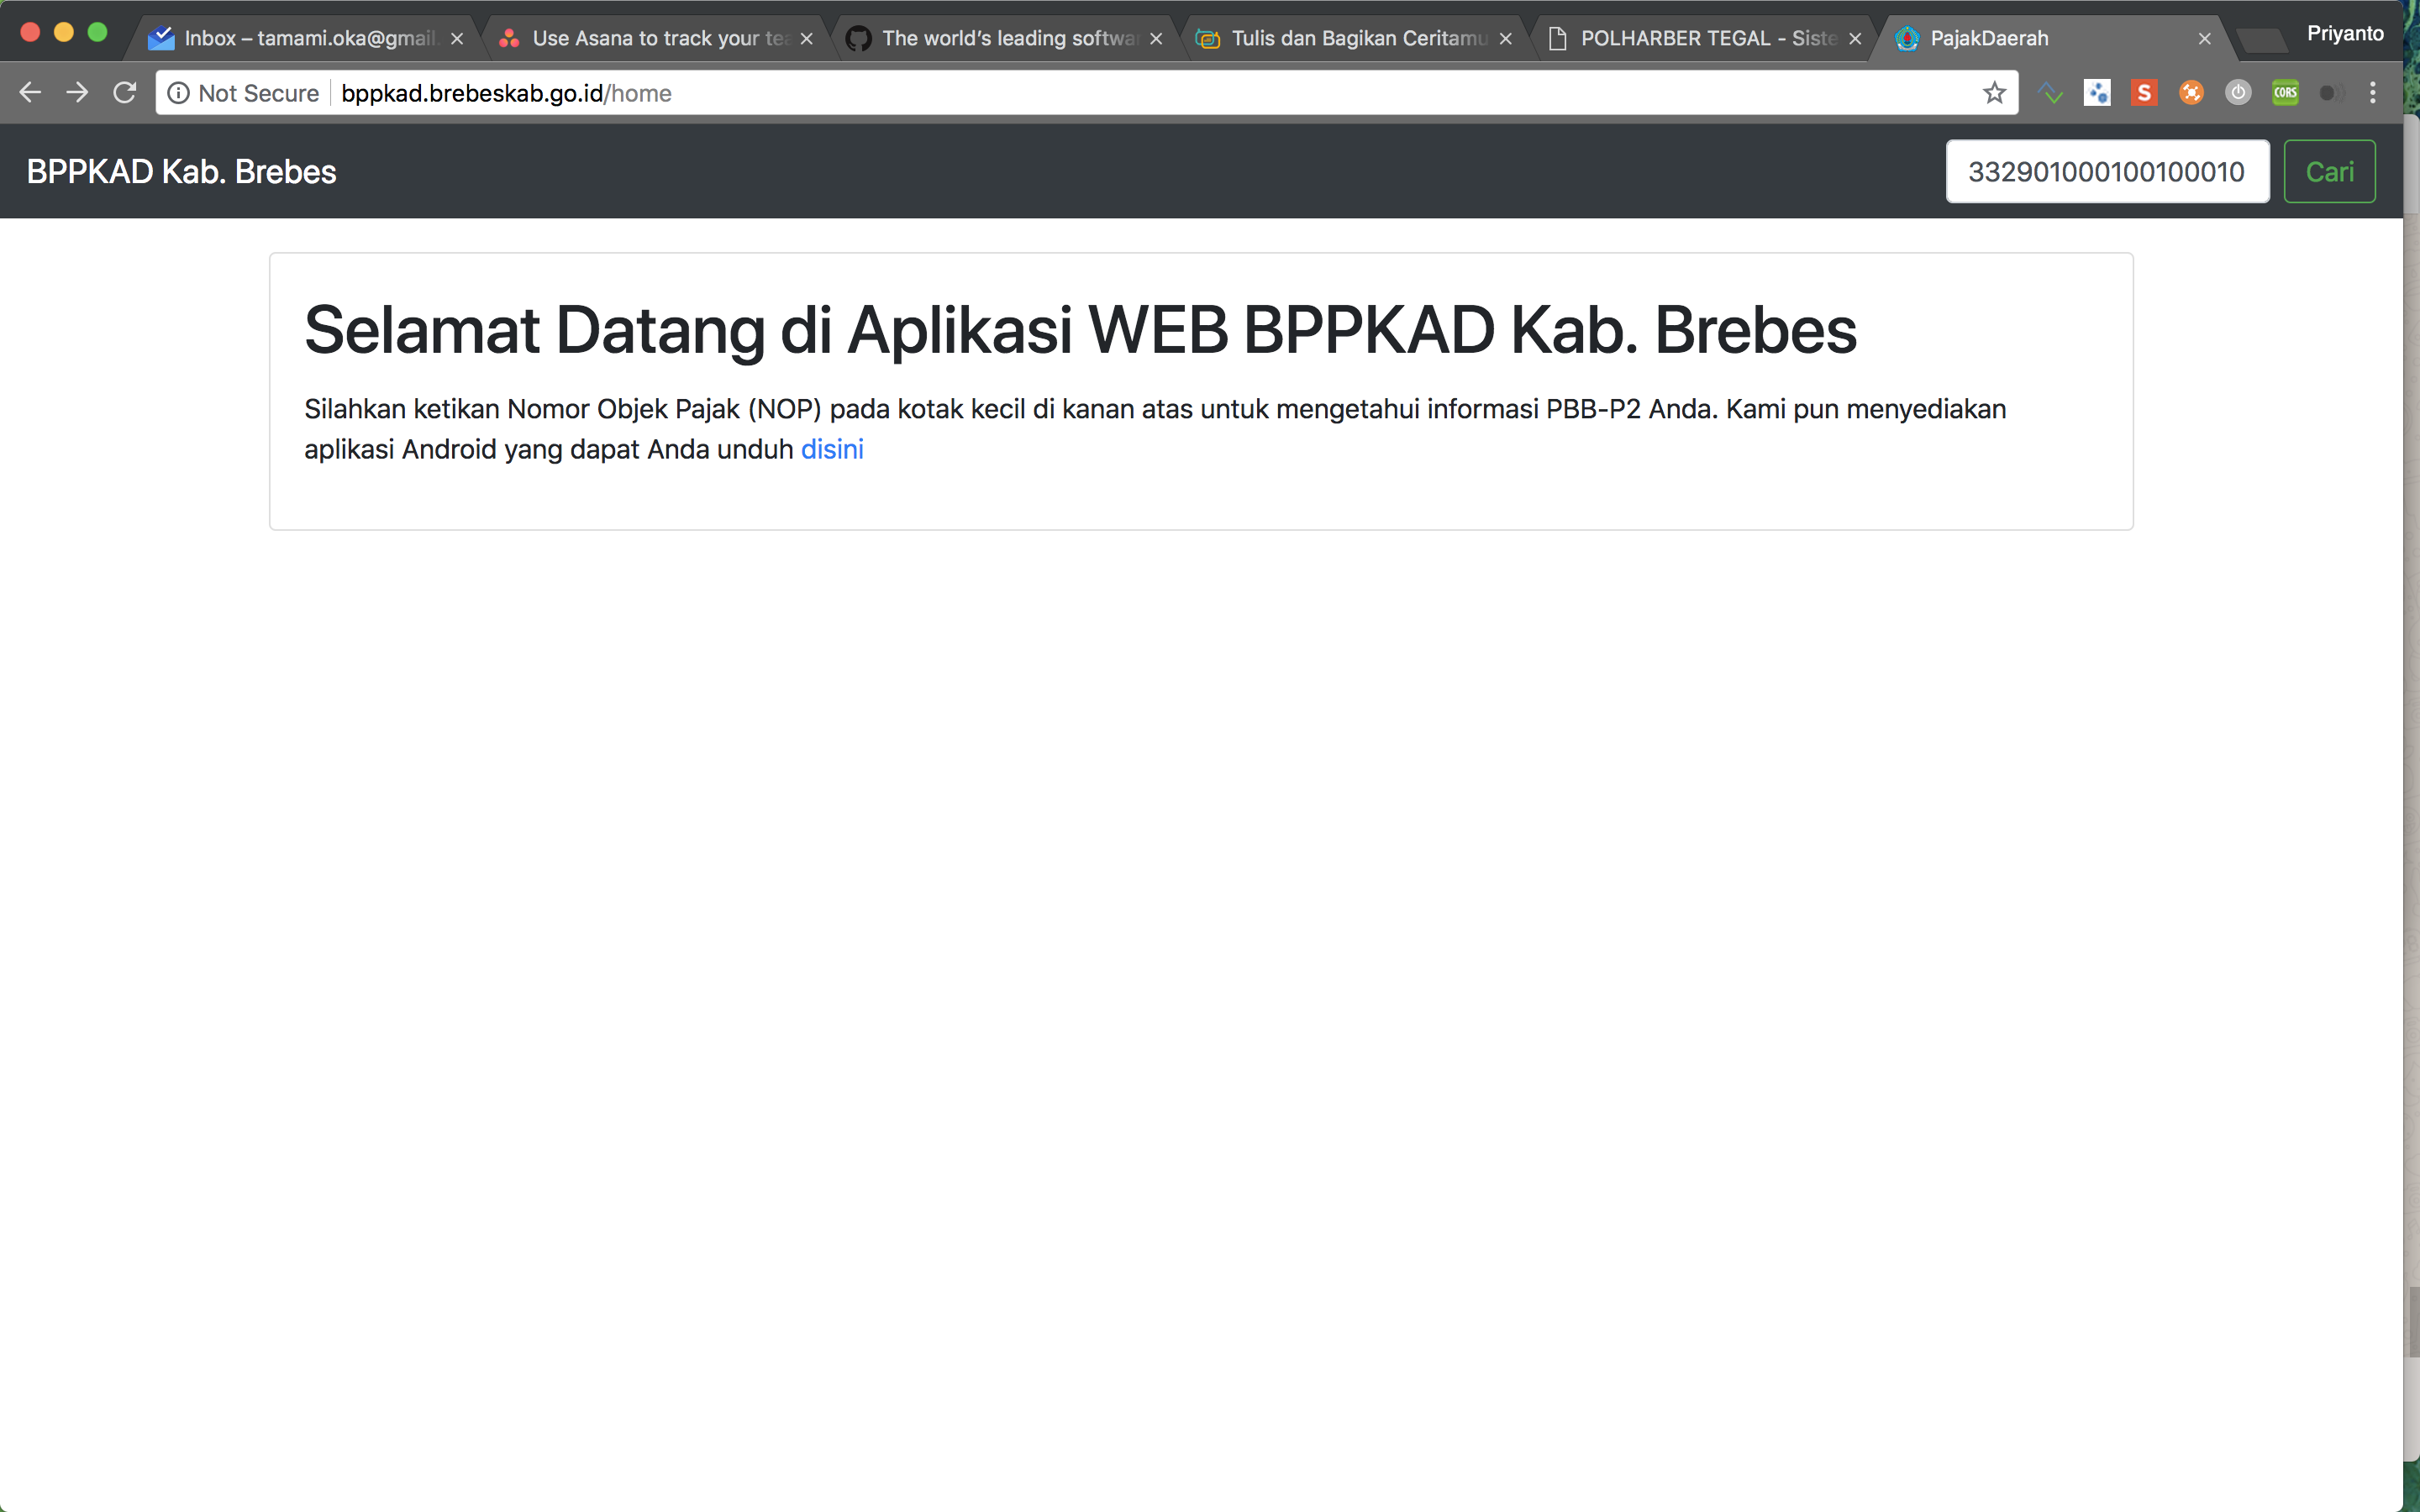
\includegraphics[width=1\textwidth]{./resources/contoh-input-nop}
	\caption{Contoh Memasukkan Nomor Objek Pajak (NOP)}
	\label{fig:contoh-nop}
\end{figure}

Setelah itu menekan tombol \textbf{Cari} di sebelahnya sehingga aplikasi akan menampilkan informasi mengenai objek pajak, subjek pajak, serta status tagihan dan pembayaran dari Surat Pemberitahuan Pajak Terhutang untuk tiap tahun pajaknya seperti gambar \ref{fig:result-info} berikut ini :

\begin{figure}[H]
	\centering
	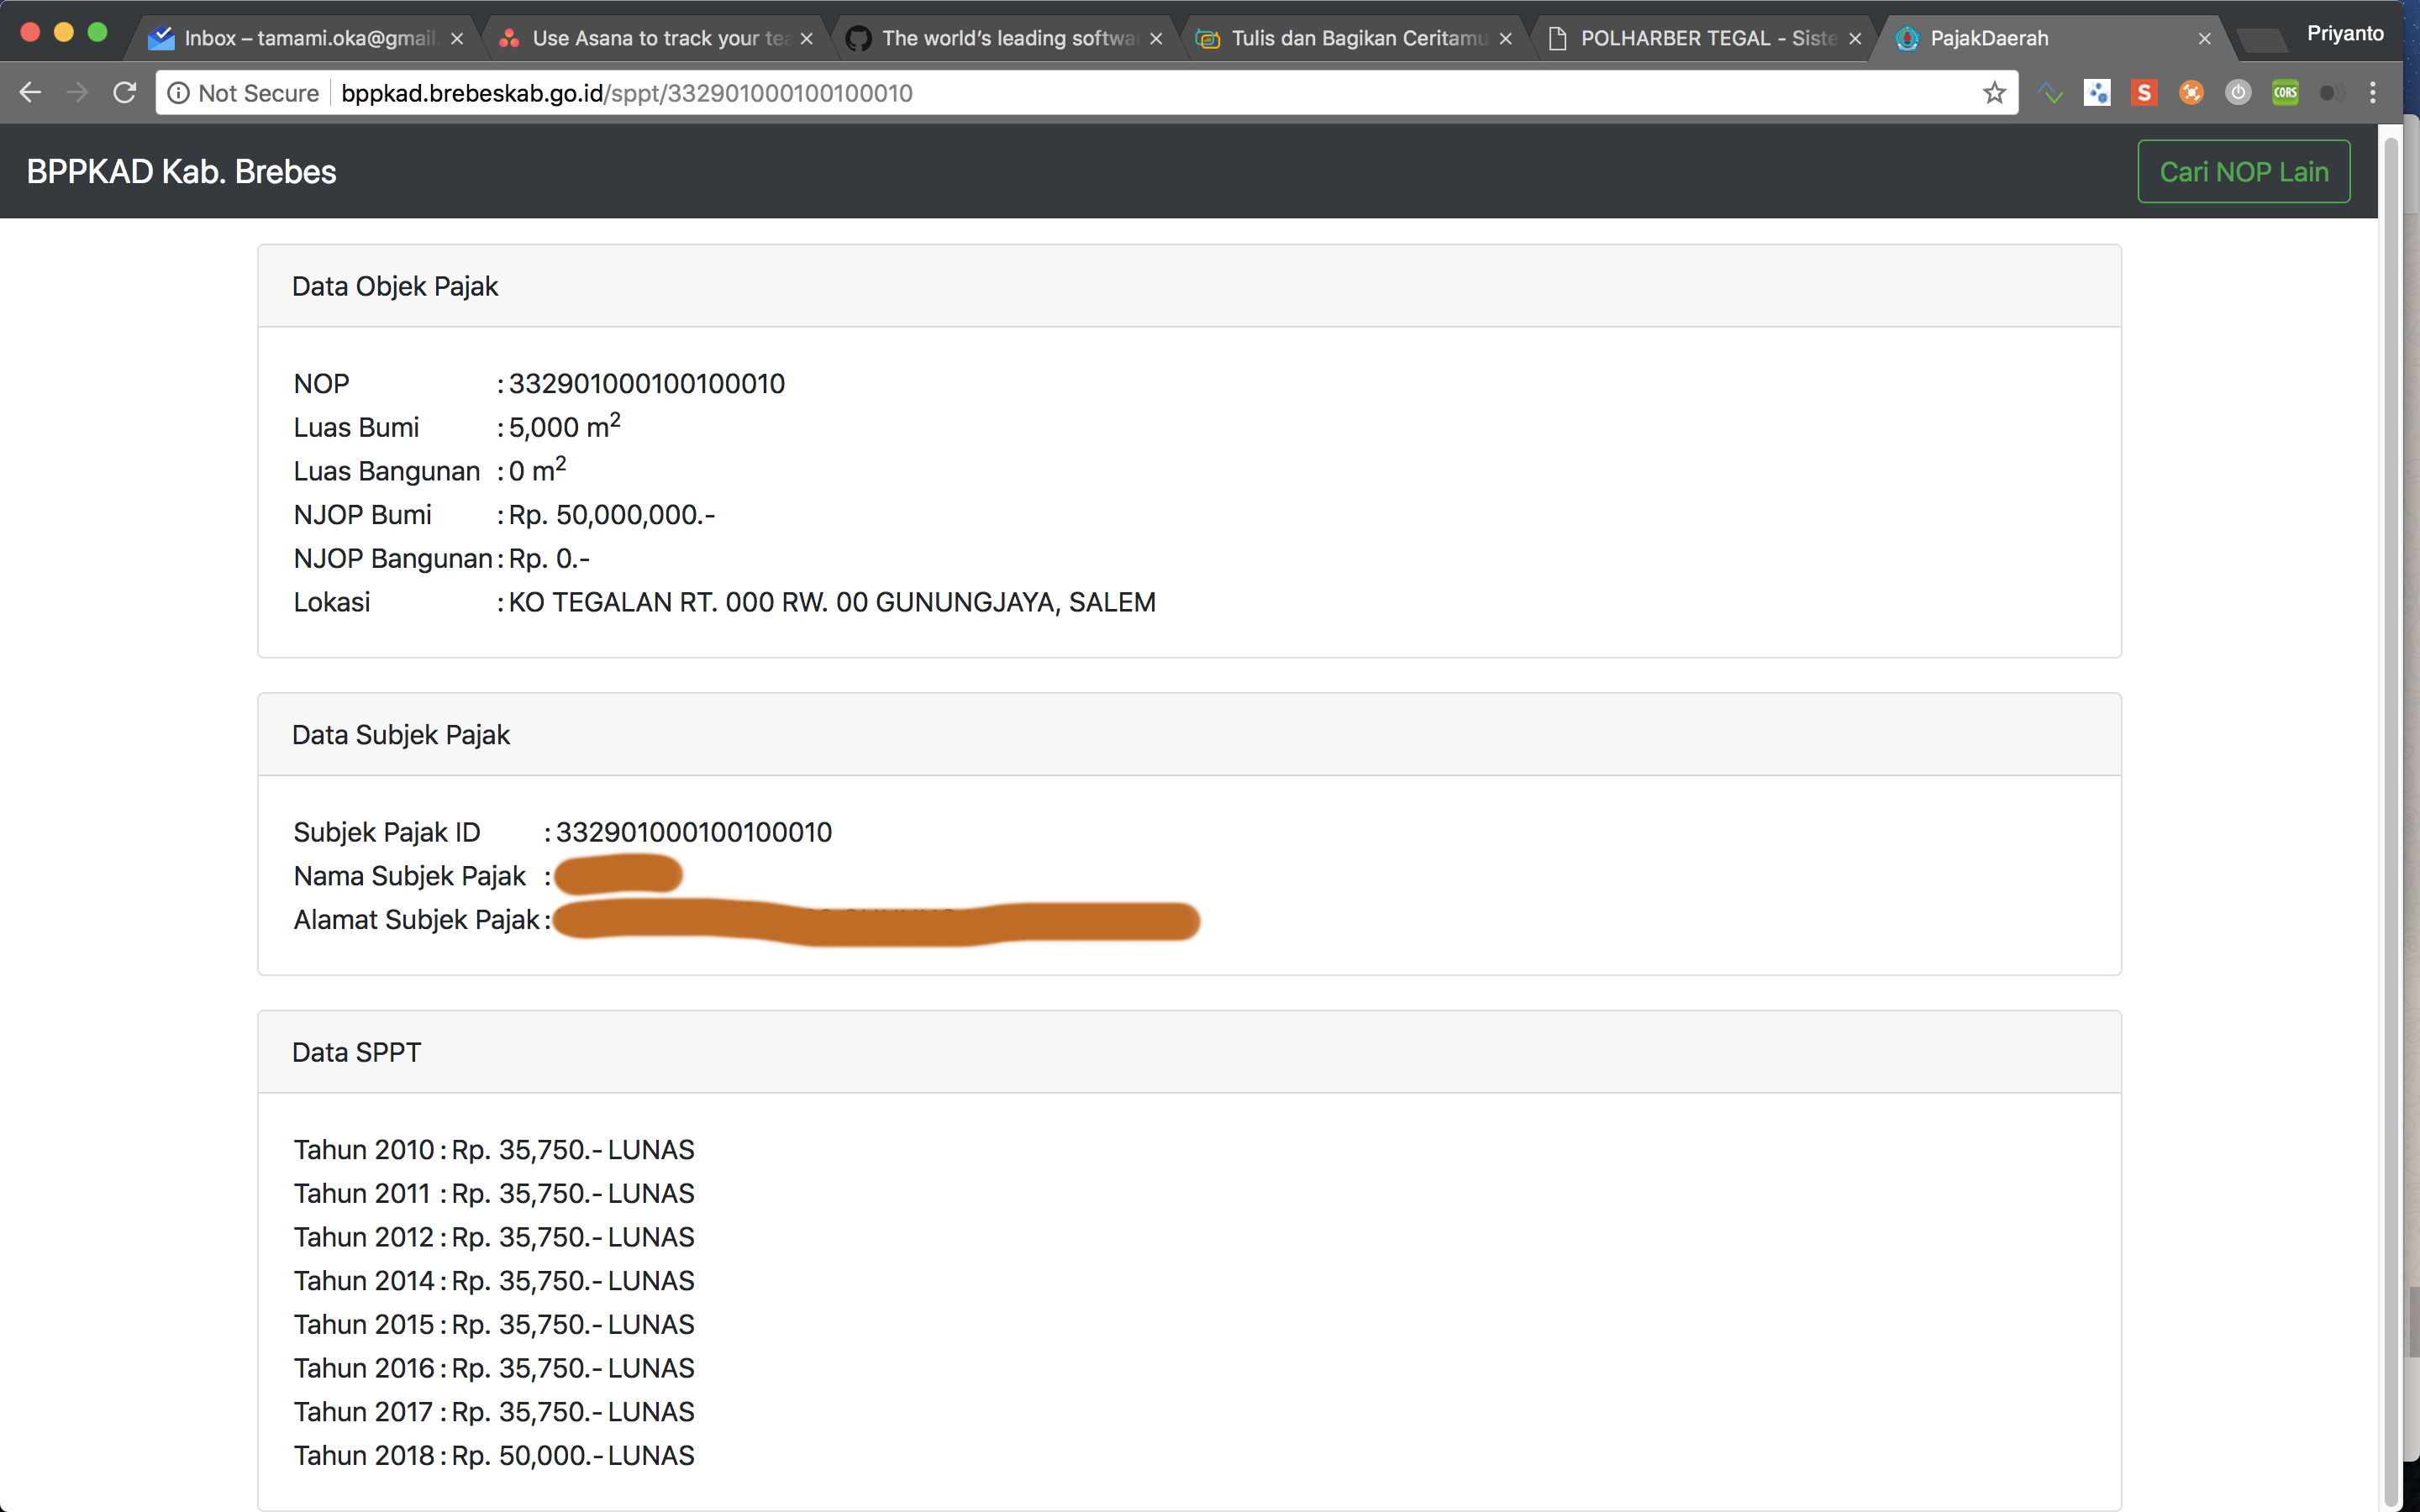
\includegraphics[width=1\textwidth]{./resources/result-info}
	\caption{Hasil Informasi Yang DIdapatkan}
	\label{fig:result-info}
\end{figure}
